\chapter{Входные и выходные данные}

Входные данные программы:
\begin{itemize}
	\item заглавная страница ресурса~---~\url{sostra.ru};
	\item количество потоков управления;
	\item количество выгружаемых страниц.
\end{itemize}

Выходные данные: директория с полученными страницами рецептов.
\clearpage

\chapter{Преобразование входных данных в выходные}

Для выгрузки страниц была написана функция представленная в листинге~\ref{lst:load}, использующая библиотеку curl~\cite{curl}, для получения ссылок на другие страницы использовались функции приведенные в листинге~\ref{lst:links}.
\begin{lstlisting}[caption={Функция выгрузки страниц}, label=lst:load]
string load_page(const string &url, set<string> &urls, queue<string> &_urls_to_handle) {
	CURL *curl = curl_easy_init();
	string result;
	if (curl) {
		curl_easy_setopt(curl, CURLOPT_WRITEFUNCTION, curl_write);
		curl_easy_setopt(curl, CURLOPT_URL, url.c_str());
		curl_easy_setopt(curl, CURLOPT_WRITEDATA, &result);
		CURLcode res_code = curl_easy_perform(curl);
		curl_easy_cleanup(curl);
		prepare_hyperlinks(result, urls, _urls_to_handle);
	}
	return result;
}
\end{lstlisting}

\begin{lstlisting}[caption={Функции выделения ссылок}, label=lst:links]
set<string> extract_hyperlinks(const string &text) {
	static const std::regex hl_regex("href=\"/(.*?)\"", std::regex_constants::icase);
	return {std::sregex_token_iterator(text.begin(), text.end(), hl_regex, 1), std::sregex_token_iterator{}};
}

void prepare_hyperlinks(const string &text, set<string> &urls, queue<string> &_urls_to_handle) {
	set<string> links = extract_hyperlinks(text);
	for (auto it = links.begin(); it != links.end();) {
		if (it->find(".ru") == -1 && it->find(".com") == -1 && it->find(".org") == -1 &&
		it->substr(0, 12) == string("recipe-book/")) {
			string new_url = string(BASE_URL) + (*it);
			set_urls_mutex.lock();
			if (urls.find(new_url) == urls.end()) {
				urls.insert(string(BASE_URL) + (*it));
				set_urls_mutex.unlock();
				queue_urls_mutex.lock();
				_urls_to_handle.push(new_url);
				queue_urls_mutex.unlock();
			} else
			set_urls_mutex.unlock();
			++it;
		}
	}
}
\end{lstlisting}

\clearpage

\chapter{Тестирование}

Для проверки работоспособности было вручную проверено содержимое выгруженных страниц. Все тесты были успешно пройдены.
\clearpage

\chapter{Примеры работы программы}

На рисунке~\ref{fig:dir} приведена директория с выгруженными страницами, представленными HTML файлами. Всего получено 191 страница рецептов.
\begin{figure}[H]
	\centering
	
\includegraphics[width=\textwidth]{dir.png}
	\caption{Директория с полученными страницами}
	\label{fig:dir}
\end{figure}

На рисунке~\ref{fig:recipe} приведена одна из выгруженных страниц с рецептами..
\begin{figure}[H]
	\centering
	
\includegraphics[width=\textwidth]{recipe.png}
	\caption{Страница с рецептом}
	\label{fig:recipe}
\end{figure}
\clearpage


\chapter{Описание исследования}

Исследовалась зависимость скорости выгрузки в терминах числа страниц в единицу времени от количества потоков. Замеры проводились для 1, 2, 4, 8, 16, 32 потоков. Выгружалось 191 страница, по три раза для каждого числа потоков, итоговое значение усреднялось.

Исследования проводились на машине со следующими характеристиками:
\begin{itemize}[label=---]
	\item процессор Intel(R) Core(TM) i5-10210U, тактовая частота 1.60 ГГц;
	\item оперативная память: 16 ГБ;
	\item операционная система: Ubuntu 22.04.4 LTS.
\end{itemize}

Результаты замеров приведены в таблице~\ref{tab:all_times}.

\begin{table}[H]
	\caption{Среднее число загружаемых страниц в единицу времени при различном числе потоков}
	\centering
	\begin{tabular}{|c|c|}
		\hline
		Число потоков & \shortstack{Среднее количество выгружаемых\\ страниц в единицу времени}\\
		\hline
		1 & 0.476693\\\hline
		2 & 1.11428\\\hline
		4 & 1.66893\\\hline
		8 & 2.41893\\\hline
		16 & 1.21408\\\hline
		32 & 1.98875\\\hline
	\end{tabular}
	\label{tab:all_times}
\end{table}

На рисунке~\ref{fig:plot} приведен график зависимости среднего числа выгружаемых страниц от числа потоков. Для визуализации данных использовалась библиотека matplotlib~\cite{plt}.

\begin{figure}[H]
	\centering
	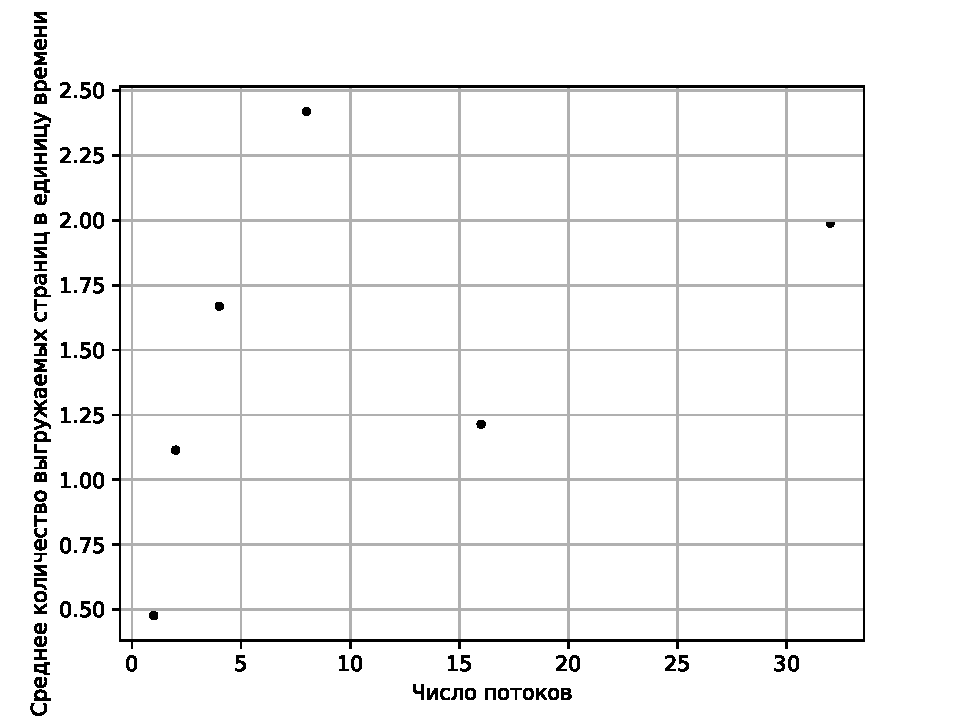
\includegraphics[width=\textwidth]{plot.pdf}
	\caption{Зависимость среднего числа выгружаемых страниц от числа потоков}
	\label{fig:plot}
\end{figure}

Из результатов исследования следует, что использование потоков для параллельного выполнения задач ускоряет работу приложения. Однако, при превышении количеством потоков числа логических ядер, дальнейшего ускорения не происходит. 
\clearpage
